\chapter{Homotopy Type Theory}

\section{Homotopical Language}

\begin{defn}
    A \textsl{pointed type} $(A,a)$ is a type $A\colon\univ$ together with a point $a\colon A$, called its \textsl{basepoint}. We write
    \[
        \univ_\sbull\defeq\sum_{A:\,\univ}A
    \]
    for the type of pointed types in the universe $\univ$.
\end{defn}

\begin{defn}
    Given a pointed type $(A,a)$, we define the \textsl{loop space} of $(A,a)$ to be the following pointed type:
    \[
        \Omega(A,a)\defeq((a\eq Aa),\fun{refl}_a).
    \]
    An element of it will be called a \textsl{loop} at $a$. For $n\colon\N$, the \textsl{$n$-fold iterated loop space} $\Omega^n(A,a)$ of a pointed type $(A,a)$ is defined recursively by:
    \begin{align*}
        \Omega^0(A,a)&\defeq(A,a)\\
        \Omega^{n+1}(A,a)&\defeq\Omega^n(\Omega(A,a)).
    \end{align*}
    An element of it will be called an \textsl{$n$-loop} or an \textsl{$n$dimensional loop} at $a$.

    Note that $\Omega^1(A,a)\equiv\Omega(A,a)$.
\end{defn}

\begin{rem}
    Recall from Exercise~\ref{exr:ap-application} that given $f\colon A\to B$, the congruence function
    \[
        \fun{ap}_f\colon\prod_{x,y\colon A}\;\prod_{p\colon x\eq Ay}f(x)\eq Bf(y)
    \]
    transforms paths in $A$ to paths in $B$. Specifically
    \[
        \fun{ap}_f(x,y,p)\colon f(x)\eq Bf(y),\quad\text{for }p\colon x\eq Ay,
    \]
    where the notation $\fun{ap}_f(x,y,p)$ is usually simplified to $\fun{ap}_f(p)$ or $\tilde f(p)$.
\if{false}    
    Moreover,
    \[
        \fun{ap}_f(\fun{refl}_x)\equiv\fun{refl}_{f(x)}
        \quad\text{and}\quad
        \fun{ap}_f(p\ct q)\eq {f(x)\eq Bf(z)}
            \fun{ap}_f(p)\ct \fun{ap}_f(q).
    \]
\fi
\end{rem}

\begin{prop}\label{prop:ap-properties}
    Let $A,B,C\colon\univ$. Given functions\/ $f\colon A\to B$ and\/ $g\colon B\to C$ and paths\/ $p\colon x\eq Ay$ and\/ $q\colon y\eq Az$, we have:
    \begin{enumerate}[a),font=\upshape]
        \item $\tilde f(\fun{refl}_x)\equiv\fun{refl}_{f(x)}$.
        \item $\tilde f(p\ct q)\eq{f(x)\eq Bf(z)}\tilde f(p)\ct\tilde f(q)$.
        \item $\tilde f(p^{-1})\eq{f(y)\eq Bf(x)}\tilde f(p)^{-1}$.
        \item $\tilde g(\tilde f(p))\eq{h(x)\eq Ch(y)}\tilde h(p)$, where $h\defeq g\circ f$.
        \item $\widetilde{\id}_A(p)\eq{x\eq Ay}p$.
    \end{enumerate}
\end{prop}

\begin{proof}${}$
    \begin{enumerate}[a)]
        \item Exercise~\ref{exr:ap-application}.
        \item Exercise~\ref{exr:ap-application}.
        
        \item First observe that
        \begin{align*}
            \tilde f(p)\ct\tilde f(p^{-1})
                &\eq{f(x)\eq Bf(x)}\tilde f(p\ct p^{-1})
                    &&\text{; by part b)}\\
                &\eq{f(x)\eq Bf(x)}\tilde f(\fun{refl}_x)
                    &&\text{; inverse law}\\
                &\equiv\fun{refl}_{f(x)}
                    &&\text{; by part a).}
        \end{align*}
        Therefore,
        \begin{align*}
            \tilde f(p)^{-1}
                &\eq{f(y)\eq Bf(x)}
                    \tilde f(p)^{-1}\ct\big(\tilde f(p) \ct\tilde f(p^{-1})\big)
                    &&\text{; right unit}\\
                &\eq{f(y)\eq Bf(x)}
                    \big(\tilde f(p)^{-1}\ct\tilde f(p)\big) \ct\tilde f(p^{-1})
                    &&\text{; associativity}\\
                &\eq{f(y)\eq Bf(x)}\tilde f(p^{-1})
                    &&\text{; left inverse.}
        \end{align*}

        \item Since $p\colon x\eq Ay$, we know that $\tilde f(p)\colon f(x)\eq Bf(y)$. Therefore,
        \[
            \tilde g(\tilde f(p))\colon g(f(x))\eq Cg(f(y)).
        \]
        Let $h\defeq g\circ f$. Note that the type of the term above is definitionally equal to $h(x)\eq C h(y)$.
        Consider the case where $p\equiv\fun{refl}_x$. We have
        \begin{align*}
            \tilde g(\tilde f(\fun{refl}_x))
                &\equiv \tilde g(\fun{refl}_{f(x)})\\
                &\equiv \fun{refl}_{g(f(x))}\\
                &\equiv \fun{refl}_{h(x)}\\
                &\equiv \tilde h(\fun{refl}_x).
        \end{align*}
        To conclude that $\tilde g(\tilde f(p))\eq{h(x)\eq Ch(y)}\tilde h(p)$, we apply path induction to the motive
        \[
            C(x,y,p)\defeq \tilde g(\tilde f(p))\eq{h(x)\eq Ch(y)}\tilde h(p),
        \]
        with the base case $c(x)\colon C(x,x,\fun{refl}_x)$ defined as $\fun{refl}_{\tilde h(\fun{refl}_x)}$.

        \item For\/ $p\equiv\fun{refl}_x$, since\/ $\id_A(x)\equiv x$, we have
        \begin{align*}
            \widetilde{\id}_A(\fun{refl}_x)
                &\equiv \fun{refl}_{\id_A(x)}\\
                &\equiv \fun{refl}_x.
        \end{align*}
        Therefore, the conclusion follows by path induction applied to the motive
        \[
            C(x,y,p)\defeq\widetilde{\id}_A(p)\eq{x\eq Ay}p
        \]
        with base case\/ $c(x)\defeq\fun{refl}_{\fun{refl}_x}\colon C(x,x,\fun{refl}_x)$.
        
    \end{enumerate}
\end{proof}

\begin{lem}\label{lem:ap-const}
    Let\/ $A, B\colon\univ$ and\/ $b\colon B$. Given the constant function\/ $f\colon A\to B$ defined by\/ $f(x)\defeq b$, for any path\/ $p\colon x\eq A y$, we have
    \[
        \fun{ap}_f(p) \eq{b\eq B b} \fun{refl}_b.
    \]
\end{lem}

\begin{proof}
    By path induction on $p$ it suffices to prove the case where $y\equiv x$ and $p\equiv \fun{refl}_x$.
    \begin{enumerate}[-]
        \item \lhs: $\fun{ap}_f(\fun{refl}_x)\equiv\fun{refl}_{f(x)}\equiv \fun{refl}_b$.
        \item \rhs: $\fun{refl}_b$.
    \end{enumerate}
    Since both sides are definitionally equal to $\fun{refl}_b$, the equality is inhabited by $\fun{refl}_{\fun{refl}_b}$.
\end{proof}

\begin{rem}\label{rem:fibration}
    Recall from classical topology that a \textsl{fibration} is a continuous map $\pi\colon E\to B$ with the homotopy-lifting property:
    \[
        \begin{tikzcd}[row sep=large, column sep=huge]
            X
                \arrow[r,"f"]
                \arrow[d,hook,"i_0"']
            &E
                \arrow[d,"\pi"] \\
            X\times I
                \arrow[r,"\forall H"']
                \arrow[ur,dashed,"\exists\tilde{H}"]
            &B
        \end{tikzcd}
    \]
    In this context, $E$ is the \textsl{total space} and $B$ the \textsl{base space} of the fibration.

    \textsl{Serre fibrations} lift paths, path homotopies, and higher-dimensional volumes. For instance, in the case of paths, the diagram above becomes:
    \[
        \begin{tikzcd}[row sep=large, column sep=large]
            \{0\}
                \arrow[r, "e_0"]
                \arrow[d, hook, "i"']
            & E
                \arrow[d, "\pi"] \\
            I
                \arrow[r, "\forall\gamma"']
                \arrow[ur, dashed, "\exists\tilde{\gamma}"]
            & B
        \end{tikzcd}
    \]
    In Homotopy Type Theory, given a type family $P\colon A\to\univ$, the first projection $\fun{\pi}_1\colon \sum_{x\colon A}P(x)\to A$ is analogous to a fibration with \textsl{total space} $\sum_{x\colon A}P(x)$ and \textsl{base space} $A$. This structural analogy is established by the lemma below.

    Given $a,b\colon A$, the type family $P$ structurally relates the fibers $P(a)$ and $P(b)$. Although a point $u\colon P(a)$ cannot be directly compared with $v\colon P(b)$ due to type mismatch, it is possible to establish a connection between the pairs $(a,u)$ and $(b,v)$ within the $\Sigma$-type. Specifically, if there exists a path $p\colon a\eq A b$, we can map $u$ along $p$ via transport to obtain an element $\fun{transport}^P(p,u)\colon P(b)$. Since this transported term inhabits the same fiber as $v$, the comparison becomes well-defined. More precisely:
    
\end{rem}

\begin{thm}{\upshape[Path Lifting Property]}\label{thm:path-lift}
    Let\/ $P\colon A\to\univ$ be a type family over\/~$A$ and let\/ $E\defeq\sum_{x\colon A}P(x)$ be its total space. Given $a,b\colon A$, there exists a function
    \[
        \fun{lift}\colon\prod_{u\colon P(a)}\;
            \prod_{p\colon a\eq Ab}
            (a,u)\eq{E}(b,\fun{transport}^P(p,u))
    \]
    \needspace{2\baselineskip}
    satisfying the following properties:
    \begin{enumerate}[i), font=\upshape]
        \item $\fun{lift}(u,p)\colon (a,u)\eq E (b,\fun{transport}^P(p,u))$.
        \item $\fun{lift}(u,\fun{refl}_a)\equiv\fun{refl}_{(a,u)}$.
        \item $\fun{ap}_{\pi_1}(\fun{lift}(u,p))\eq{a\eq Ab}p$.
    \end{enumerate}
    where\/ $\pi_1\colon E\to A$ denotes the first projection.\footnotemark
\end{thm}
\footnotetext{Since\/ $\pi_1$ maps the total space to the base type\/ $A$, the functorial action\/ $\fun{ap}_{\pi_1}$ projects paths in\/ $E$ to paths in\/ $A$.}


\begin{proof}
    Consider the motive family\/ $C\colon\prod_{x\colon A}(a\eq Ax)\to\univ$, defined by
    \[
        C(x,p)\defeq(a,u)\eq E(x,\fun{transport}^P(p,u)).
    \]
    Since\/ $\fun{transport}^P(\fun{refl}_a,u)\equiv u$, we have
    \[
        C(a,\fun{refl}_a)\equiv(a,u)\eq E(a,u),
    \]
    and we can specify the base case\/ $c\defeq\fun{refl}_{(a,u)}$ to define, by \nref{lpar:based-path-induction},
    \[
        \fun{lift}(u,p)\defeq\fun{ind}'_{\eq A}(a,C,c,x,p).
    \]
    We can use based path induction again to verify that
    \[
        \fun{ap}_{\fun{\pi}_1}(\fun{lift}(u,p)) \eq{a\eq Ax} p.
    \]
    For the base case, we know definitionally that\/ $\fun{lift}(u,\fun{refl}_a) \equiv \fun{refl}_{(a,u)}$. Thus,
    \[
        \fun{ap}_{\fun{\pi}_1}(\fun{lift}(u,\fun{refl}_a))
        \equiv \fun{ap}_{\fun{\pi}_1}(\fun{refl}_{(a,u)})
        \equiv \fun{refl}_{\pi_1(a,u)}
        \equiv \fun{refl}_a.
    \]
\end{proof}

\begin{rem}\label{rem:section-type}
    The lemma can be represented by the following diagram, where the horizontal arrows represent paths ---i.e., terms of the propositional equalities between their ends--- and the vertical arrows, functions:
    \[
        \begin{tikzcd}[row sep=large, column sep=huge]
            (a,u)
                \arrow[r,"{\fun{lift}(u,p)}"]
                \arrow[d,"\pi_1"']
            &(x, \fun{transport}^P(p,u))
                \arrow[d,"\pi_1"] \\
            a
                \arrow[r,"p"']
            &x
        \end{tikzcd}
        \qquad;\ u\colon P(a),\;p\colon a\eq Ax.
    \]
    Note also that a term $f\colon\prod_{x\colon A}P(x)$ can be regarded as a \textsl{section} of the fibration induced by~$P$.
\end{rem}

\begin{ntn}\label{ntn:p_*}
    When\/ $P$ is clear from the context we will simply write
    \[
        p_*(u)\defeq\fun{transport}^P(p,u)\colon P(x).
    \]
    In particular,
    \begin{equation}\label{eq:refl-*}
        (\fun{refl}_a)_*(u)\equiv u.
    \end{equation}
\end{ntn}

\begin{defn}\label{defn:sec}
    Let $A,B\colon\univ$. Given $b\colon B$ we define the \textsl{section} function
    \[
        \fun{sec}_b\colon A\to A\times B,\quad a\mapsto(a,b).
    \]
    Note that
    \begin{align*}
        \pi_1\circ\fun{sec}_b
            &\equiv\pi_1(\lambda x.\,(x,b))
            \equiv\lambda x.\,\pi_1((x,b))
            \equiv\lambda x.\,x
            \equiv\id_A.\\
        \pi_2\circ\fun{sec}_b
            &\equiv\pi_2(\lambda x.\,(x,b)
            \equiv\lambda x.\,\pi_2((x,b)
            \equiv\lambda x.\,b.
    \end{align*}
\end{defn}

\begin{rem}\label{rem:sec-lift}
    In the particular case where $P$ is a constant family $P(x)\equiv B$ for $x\colon A$, given $p\colon a\eq Aa'$, we have
    \begin{enumerate}[i)]
        \item $\fun{lift}(b,p)\eq{(a,b)\eq{A\times B}(a',b)}\fun{ap}_{\fun{sec}_b}(p)$,
        \item $\fun{lift(b,\fun{refl}_a})\equiv\fun{refl}_{(a,b)}$, and
        \item $\fun{ap}_{\pi_1}(\fun{lift}(b,p))\eq{a\eq Aa'}p$.
    \end{enumerate}
    In fact, the equality of part~i) follows from part~ii) by induction on $p$.
    \[
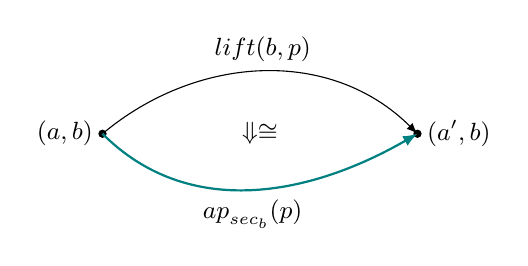
\begin{tikzpicture}[scale=1, >=stealth, font=\small]
    % Points
    \coordinate (start) at (0,0);
    \coordinate (end) at (4,0);

    \fill (start) circle (1.5pt) node[left] {$(a,b)$};
    \fill (end) circle (1.5pt) node[right] {$(a',b)$};

    % Top Path: lift(b,p)
    \draw[-latex,] (start) to[out=40, in=135] 
        node[midway, above,black] {$\fun{lift}(b,p)$} (end);

    % Bottom Path: ap(sec_b, p)
    \draw[-latex, thick, teal] (start) to[out=-45, in=-150] 
        node[midway, below,black] {$\fun{ap}_{\fun{sec}_b}(p)$} (end);

    % The 2-path (Equality)
    \node at (2,0) {$\Downarrow \cong$};
\end{tikzpicture}
    \]
\end{rem}

\begin{lem}{\upshape[Dependent map]}
    Let\/ $P\colon A\to\univ$. If\/ $f\colon\prod_{x\colon A}P(x)$, then there is a map
    \[
        \fun{apd}_f\colon\prod_{x,y\colon A}\;
            \prod_{p\colon x\eq Ay}
                p_*(f(x))\eq{P(y)}f(y)
    \]
    satisfying $\fun{apd}_f(\fun{refl}_x)\equiv\fun{refl}_{f(x)}$.
\end{lem}

\begin{proof}
    Fix $a\colon A$ and consider the motive
    \begin{align*}
        C&\colon\prod_{a\colon A}(a\eq Ax)\to\univ\\
        C(x,p)&\defeq p_*(f(a))\eq{P(x)}f(x).
    \end{align*}
    Since
    \begin{align*}
        C(a,\fun{refl}_a)
            &\equiv (\fun{refl}_a)_*(f(a))\eq{P(a)}f(a)\\
            &\equiv f(a)\eq{P(a)}f(a)
                &&\text{; \eqref{eq:refl-*}},
    \end{align*}
    we can specify $c\defeq\fun{refl}_{f(a)}$ and obtain $\fun{apd}_f$ by based path induction.
\end{proof}

\begin{lem}
    If\/ $P \colon A \to \univ$ is defined by\/ $P(x) :\equiv B$ for a fixed\/ $B \colon \univ$, then for any\/ $x, y \colon A$ and\/ $p \colon x \eq A y$ and\/ $b \colon B$ we have a path
    \[
        \fun{transportconst}^B_p(b) \colon \fun{transport}^P(p, b) \eq B b
    \]
    satisfying\/ $\fun{transportconst}^B_{\fun{refl}_x}\defeq\lambda b.\,\fun{refl}_b$.
\end{lem}

\begin{proof}
    See Exercise \ref{exr:constant-fibration}.
\end{proof}

\begin{lem}
    Let\/ $f \colon A \to B$ and define the constant family\/ $P \colon A \to \univ$ by\/ $P(x) :\equiv B$. For any path\/ $p \colon x \eq A y$, we have
    \[
        \fun{apd}_f(p)\eq{p_*(f(x))\eq B f(y)}
            \fun{transportconst}^B_p(f(x))\ct\fun{ap}_f(p).
    \]
\end{lem}

\begin{proof}
    Fix\/ $a\colon A$ and let\/ $C\colon\prod_{x\colon A}(a\eq Ax)\to\univ$ be defined by
    \[
        C(x,p)\defeq\fun{apd}_f(p)\eq{p_*(f(a))\eq Bf(x)}
            \fun{transportconst}^B_p(f(a))\ct\fun{ap}_f(p).
    \]
    To verify the base case:
    \begin{align*}
        C(a,\fun{refl}_a)
            &\equiv\fun{apd}_f(\fun{refl}_a)
                \eq{(\fun{refl}_a)_*(f(a))\eq Bf(a)}
                \fun{transportconst}^B_{\fun{refl}_a}(f(a))
                \ct\fun{ap}_f(\fun{refl}_a)\\
            &\equiv\fun{refl}_{f(a)}
                \eq{f(a)\eq Bf(a)}
                \fun{refl}_{f(a)}\ct\fun{refl}_{f(a)}\\
            &\equiv \fun{refl}_{f(a)}
                \eq{f(a)\eq Bf(a)}
                \fun{refl}_{f(a)}.
    \end{align*}
    Therefore, we can specify the base case\/ $c\defeq\fun{refl}_{\fun{refl}_{f(a)}}$ to complete the proof by based path induction.
\end{proof}

\begin{rem}
    We can represent the previous lemma in a propositionally commutative path diagram, where ``composition'' means concatenation:
    \[
        \begin{tikzcd}[column sep=2.8cm,row sep=1.5cm]
            p_*(f(x))
                    \arrow[r,"\fun{transportconst}^B_p(f(x))"]
                    \arrow[rd,"\fun{apd}_f(p)"']&f(x)
                    \arrow[d,"\fun{ap}_f(p)"]\\
                &f(y)
        \end{tikzcd}
    \]    
\end{rem}

\begin{lem}
    Given\/ $P\colon A\to\univ$, $p\colon x\eq Ay$ and, $q\colon y \eq Az$, and\/ $u\colon P(x)$, we have
    \[
        q_*(p_*(u))\eq{P(z)}(p\ct q)_*(u).
    \]
\end{lem}

\begin{proof}
    Fix $x\colon A$. We proceed by based path induction on $p\colon x\eq A y$. The motive of the induction is the family of types $D\colon \prod_{y\colon A} (x\eq A y)\to \univ$ defined by
    \[
        D(y, p) \defeq \prod_{u\colon P(x)}\; \prod_{z\colon A}\; \prod_{q\colon y\eq A z}
            q_*(p_*(u)) \eq{P(z)} (p\ct q)_*(u).
    \]
    We must construct a term of type $D(x, \fun{refl}_x)$. Substituting $y$ with $x$ and $p$ with $\fun{refl}_x$, the goal becomes
    \[
        \prod_{u\colon P(x)}\;
            \prod_{z\colon A}\;
            \prod_{q\colon x\eq Az} 
                q_*((\fun{refl}_x)_*(u))\eq{P(z)}
                    (\fun{refl}_x\ct q)_*(u).
    \]
    Using the definitional equalities $(\fun{refl}_x)_*(u) \equiv u$ and $\fun{refl}_x\ct q \equiv q$, this reduces to
    \[
        \prod_{u\colon P(x)}\;
            \prod_{z\colon A}\;
                \prod_{q\colon x\eq Az}
                    q_*(u)\eq{P(z)}q_*(u),
    \]
    which is inhabited by $\lambda u,z,q.\,\fun{refl}_{q_*(u)}$.
\end{proof}

\begin{lem}
    For a function\/ $f \colon A \to B$, a type family\/ $P \colon B \to \univ$, and any\/ $p \colon x \eq A y$ and\/ $u \colon P(f(x))$, we have
    \[
        \fun{transport}^{P\circ f}(p,u) \eq{P(f(y))}
            \fun{transport}^P(\fun{ap}_f(p),u).
    \]
\end{lem}

\begin{proof}
    We proceed by path induction on $p$. Define the motive
    \[
        C\colon \prod_{y\colon A} (x\eq A y)\to \univ
    \]
    by
    \[
        C(y,p) \defeq
            \prod_{u\colon P(f(x))}
                \fun{transport}^{P\circ f}(p,u) \eq{P(f(y))}
                    \fun{transport}^P(\fun{ap}_f(p),u).
    \]
    Evaluating at the base case, we have
    \begin{align*}
        C(x,\fun{refl}_x)
            &\equiv \prod_{u\colon P(f(x))}
                \fun{transport}^{P\circ f}(\fun{refl}_x,u)
                    \eq{P(f(x))}
                    \fun{transport}^P(\fun{ap}_f(\fun{refl}_x),u) \\
            &\equiv \prod_{u\colon P(f(x))}
                u \eq{P(f(x))}
                    \fun{transport}^P(\fun{refl}_{f(x)},u) \\
            &\equiv \prod_{u\colon P(f(x))}
                u \eq{P(f(x))} u,
    \end{align*}
    which is inhabited by $\lambda u\colon P(f(x)).\,\fun{refl}_u$.
\end{proof}

\begin{lem}
    For\/ $P, Q \colon A \to \univ$, a function family\/ $f \colon \prod_{x\colon A} P(x) \to Q(x)$, and any\/ $p \colon x \eq A y$ and\/ $u \colon P(x)$, we have
    \[
        \fun{transport}^Q(p,f_x(u))\eq{Q(y)}
            f_y(\fun{transport}^P(p,u)).
    \]
\end{lem}

\begin{proof}
    To use based path induction on $p$, fix $a\colon A$ and consider the motive 
    \begin{align*}
        C&\colon\prod_{x\colon A}(a\eq Ax)\to\univ\\
        C(x,p)&\defeq\prod_{u\colon P(a)}
            \fun{transport}^Q(p,f_a(u))\eq{Q(x)}
                f_x(\fun{transport}^P(p,u)).
    \end{align*}
    For the base case we obtain
    \begin{align*}
        C(a,\fun{refl}_a)
            &\equiv\prod_{u\colon P(a)}
                \fun{transport}^Q(\fun{refl}_a,f_a(u))\eq{Q(a)}
                    f_a(\fun{transport}^P(\fun{refl}_a,u))\\
            &\equiv\prod_{u\colon P(a)}f_a(u)\eq{Q(a)}f_a(u),
    \end{align*}
    which is inhabited by $\lambda u\colon P(a).\,\fun{refl}_{f_a(u)}$.
\end{proof}

%
%
\begin{defn}
    Given a function\/ $f\colon A\to B$ and a point\/ $a\colon A$, the \textsl{induced map on loops} is the function
    \[
        \Omega f \colon \Omega(A, a) \to \Omega(B, f(a))
    \]
    defined by
    \[
        \Omega f(p) \defeq \fun{ap}_f(p).
    \]
    Note that by part a) of the previous lemma, we have\/ $\Omega f(\fun{refl}_a) \equiv \fun{refl}_{f(a)}$, meaning that\/ $\Omega f$ preserves the basepoint definitionally.
\end{defn}

\[
    \begin{tikzcd}[column sep=huge,row sep=large]
        a
                \arrow[r,bend left=45,"p"{name=U1}]
                \arrow[r,bend right=45,"q"'{name=D1}]
            &b
                \arrow[r,bend left=45,"r"{name=U2}]
                \arrow[r,bend right=45,"s"'{name=D2}]
            &c
                \arrow[Rightarrow,from=U1,to=D1,"\alpha",
                    shorten <= 8pt,shorten >= 8pt]
                \arrow[Rightarrow,from=U2,to=D2,"\beta",
                    shorten <= 8pt,shorten >= 8pt]
    \end{tikzcd}
\]

\begin{thm} {\upshape[Eckmann-Hilton]}
    The composition operation on the second loop space
    \[
        \Omega^2(A)\times\Omega^2(A)\to\Omega^2(A)
    \]
    is commutative: $\alpha\ct\beta=\beta\ct\alpha$, for any\/ $\alpha,\beta\colon\Omega^2(A)$.
\end{thm}

\section{Function Homotopies}

\begin{ntn}
    Given a type family $P\colon A\to\univ$, we will sometimes denote type of sections\footnote{Remark \ref{rem:section-type}.} $\prod_{x\colon A}P(x)$ by $\Gamma(P)$.
\end{ntn}

\begin{defn}
    Given two sections\/ $f,g\colon\prod_{x\colon A}P(x)$ of a family\/ $P\colon A\to\univ$, a \textsl{homotopy} from\/ $f$ to\/ $g$ is a dependent function of type
    \[
        f\sim g\defeq\prod_{x\colon A}f(x)\eq\univ g(x).
    \]
\end{defn}

\begin{xmpl}\label{xmpl:uniq-as-homotopy}${}$    
    As defined in \nref{lpar:Pi-types-over-product},
    \[
        \fun{uniq}_{A\times B}
            \colon(\pi_1,\pi_2)\sim\id_{A\times B},
    \]
    where $(\pi_1,\pi_2)\defeq\lambda x.\,(\pi_1(x),\pi_2(x))$.
\end{xmpl}

\begin{prop}\label{prop:homotopy-equivalence-relation}
    % Define a length to store the width of the longest subscript.
    \newlength{\maxsubwidth}
    % Measure the widest subscript (the third one) in scriptstyle (standard for limits).
    \settowidth{\maxsubwidth}{$\scriptstyle f,g,h\colon\Gamma(P)$}
    % Define a helper command to wrap the subscript in a centered box of that fixed width.
    \newcommand{\alignedprod}[1]{\prod_{\makebox[\maxsubwidth][c]{$\scriptstyle #1$}}}
    Homotopy is an equivalence relation on each dependent function type\/ $\prod_{x\colon A}P(x)$. That is, we have elements of the types
    \begin{align*}
        &\alignedprod{f\colon\Gamma(P)}
            f\sim f\\
        &\alignedprod{f,g\colon\Gamma(P)}
            (f\sim g)\to(g\sim f)\\
        &\alignedprod{f,g,h\colon\Gamma(P)}
            (f\sim g)\to(g\sim h)\to(f\sim h).
    \end{align*}
\end{prop}

\begin{proof}
    We have the following inhabitants for each of the\/ $\Pi$-types:
    \begin{itemize}
        \item \textit{Reflexivity:}\/ $\lambda f\colon\Gamma(P).\,\lambda x\colon A.\,\fun{refl}_{f(x)}$.
        \item \textit{Symmetry:}\/ $\lambda f,g\colon\Gamma(P).\,\lambda \eta\colon f\sim g.\,\lambda x\colon A.\,\eta(x)^{-1}$.
        \item \textit{Transitivity:}\/ $\lambda f,g,h\colon\Gamma(P).\,\lambda\eta\colon f\sim g.\,\lambda\vartheta\colon g\sim h.\,\lambda x\colon A.\,\eta(x)\ct\vartheta(x)$.
    \end{itemize}
\end{proof}

\begin{prop}\label{prop:ap-as-functor}
    Let\/ $f\colon A\to B$ and\/ $g\colon B\to C$ be functions. Then,
    \begin{enumerate}[a),font=\upshape]
        \item $\fun{ap}_f(p\ct q)\eq B\fun{ap}_f(p)\ct\fun{ap}_f(q)$.
        \item $\fun{ap}_f(p^{-1})\eq B\fun{ap}_f(p)^{-1}$.
        \item $\fun{ap}_{g\circ f}(p)\eq C\fun{ap}_g(\fun{ap}_f(p))$.
        \item $\fun{ap}_{\fun{id}_A}(p)\eq Ap$.
    \end{enumerate}
\end{prop}

\needspace{2\baselineskip}
\begin{proof}${}$
    \begin{enumerate}[a)]
        \item See Exercise~\ref{exr:ap-application}.
        
        \item By path induction on $p$, we reduce to the case where $p\equiv\fun{refl}_x$. We must show:
        \[
            \fun{ap}_f(\fun{refl}_x^{-1})
            \eq B
            \fun{ap}_f(\fun{refl}_x)^{-1},
        \]
        which holds since both sides compute to $\fun{refl}_{f(x)}$.
        
        \item By path induction on $p$, we reduce to the case where $p\equiv\fun{refl}_x$.
        \begin{align*}
            \fun{ap}_{g\circ f}(\fun{refl}_x)
                &\equiv\fun{refl}_{g(f(x))}\\
                &\equiv\fun{ap}_g(\fun{refl}_{f(x)})\\
                &\equiv \fun{ap}_g(\fun{ap}_f(\fun{refl}_x)).
        \end{align*}
        
        \item By path induction on $p$, we reduce to the case where $p\equiv\fun{refl}_x$, where the equality holds because
        \[
        \fun{ap}_{\fun{id}_A}(\fun{refl}_x)\equiv\fun{refl}_x.
        \]
    \end{enumerate}
\end{proof}

\begin{rem}\label{rem:types-as-categories} {\upshape[Types as categories]}
    Types admit different interpretations; depending on the circumstances we can see them as sets, propositions, spaces. Another way to think of types is as categories. In this analogy we have
    \begin{description}[font=\normalfont\scshape]
        \item[Objects.] These are the elements of the type: $x,y\colon A$ represent the objects that populate the category $A$.

        \item[Arrows.] Given two objects $x,y\colon A$, an arrow is a path $p\colon x\eq Ay$.

        \item[Composition.] Composition is concatenation. Note however that if $p\colon x\eq Ay$ and $q\colon y\eq Az$, then $p\ct q\colon x\eq Az$ is denoted in the reverse order when compared to categorical composition. We could also consider $q\circ p\defeq p\ct q$. Note that concatenation is propositionally associative.

        \item[Identity.] Given $x\colon A$ the identity for concatenation is $\fun{refl}_x$. Note that $\fun{refl}_x$ is the propositional unit of concatenation. 

        \item[Functors.] A function $f\colon A\to B$ acts as a functor between the corresponding categories:
        \begin{center}
            \begin{tabular}{lll}
                \small
                \textbf{Feature}
                    &\textbf{Domain}
                    &\textbf{Codomain}\\
                \hline\rule{0mm}{3.5mm}\small
                Objects
                    &$x\colon A$
                    &$f(x)\colon B$\\[0.7mm]
                \small
                Morphisms
                    &$p\colon x\eq A y$
                    &$\tilde f(p)\colon f(x)\eq Bf(y)$\\[0.7mm]
                \small
                Composition
                    &$p\ct q$
                    &$\tilde f(p)\ct\tilde f(q)$
            \end{tabular}
        \end{center}

        \item[Natural transformations.] These are the homotopies: given $f,g\colon A\to B$, a natural transformation between them is an inhabitant of the homotopy type $\eta\colon f\sim g$. To see this we need to show the (propositional) commutativity of the square
        \begin{equation}\label{eq:nat-transformation}
            \begin{tikzcd}
                f(x)
                        \arrow[r,"\tilde f(p)"]
                        \arrow[d,"\eta_x"']
                    &f(y)
                        \arrow[d,"\eta_y"]\\
                g(x)
                        \arrow[r,"\tilde g(p)"']
                    &g(y)
            \end{tikzcd}
        \end{equation}
        i.e., for every $p\colon x\eq Ay$, the type
        \begin{align*}
            \tilde f(p)\ct\eta_y\eq B\eta_x\ct\tilde g(p)
        \end{align*}
        is inhabited. This follows by based path induction on $p$ using the motive $C\colon\prod_{y\colon A}(x\eq Ay)\to\univ$ defined by
        \[
            C(y,p)\defeq
                \tilde f(p)\ct\eta_y\eq B\eta_x\ct\tilde g(p),
        \]
        which satisfies
        \begin{align*}
            C(x,\fun{refl}_x)
                &\defeq\tilde f(\fun{refl}_x)\ct\eta_x
                    \eq B\eta_x\ct\tilde g(p)\\
                &\equiv\fun{refl}_{f(x)}\ct\eta_x
                    \eq B\eta_x\ct\fun{refl}_{g(x)}\\
                &\equiv \eta_x\eq B\eta_x\ct\fun{refl}_{g(x)}.
        \end{align*}
        By Lemma~\ref{lem:right-unit-law}, $\fun{unit}_r(\eta_x)\colon\eta_x\ct\fun{refl}_{g(x)}\eq B\eta_x$. Hence, $\fun{unit}_r(\eta_x)^{-1}$ is an inhabitant $C(x,\fun{refl}_x)$.\footnote{To achieve independence of our definition of concatenation, we could also have used the left unit law $\fun{unit}_l$, that satisfies $\fun{unit}_l(p)\colon\fun{refl}_x\ct p\eq Ap$, arriving at $\fun{unit}_l(\eta_x)\ct\fun{unit}_r(\eta_x)^{-1}$.}
    \end{description}
\end{rem}

\begin{prop}
    Let\/ $\eta\colon f\sim\id_A$ be a homotopy, with\/ $f\colon A\to A$. Then for any\/ $x\colon A$ we have
    \[
        \eta_{f(x)}\eq A\tilde f(\eta_x).
    \]
\end{prop}

\begin{proof}
    By \eqref{eq:nat-transformation}, we have a commutative path diagram
    \[
        \begin{tikzcd}
        f(f(x))
                \arrow[r,"\tilde f(\eta_x)"]
                \arrow[d,"\eta_{f(x)}"']
            &f(x)
                \arrow[d,"\eta_x"]\\
        f(x)
                \arrow[r,"\eta_x"']
            &x
        \end{tikzcd}
    \]
    where, according to Lemma~\ref{prop:ap-as-functor}, we have replaced $\widetilde\id_A(\eta_x)$ with $\eta_x$. The conclusion follows from concatenation with $\eta_x^{-1}$.
\end{proof}

\begin{prop}{\upshape[Whiskering]}\label{prop:whiskering}
    The homotopy relation is compatible with composition:
    \begin{description}[font=\normalfont\scshape]
        \item[Right:] Given\/ $\eta\colon f\sim g$ and a right composable function\/ $h$, we have
        \[
            \eta\cdot h\defeq\lambda z.\,\eta(h(z))\colon f\circ h\sim g\circ h.
        \]
        \item[Left:] Given a left composable function\/ $h$ and\/ $\eta\colon f\sim g$, we have
        \[
            h\cdot\eta\defeq\lambda x.\,\fun{ap}_h(\eta(x))\colon h\circ f\sim h\circ g.
        \]
    \end{description}
\end{prop}

\begin{proof}
    Assume that\/ $f,g\colon A\to B$ and let\/ $\eta\colon f\sim g$ be a homotopy.

    First, consider the case where\/ $h\colon C\to A$. Given\/ $z\colon C$, we have\/ $h(z)\colon A$ and therefore a path\/ $\eta(h(z))\colon f(h(z))\eq B g(h(z))$. Hence, the term\/ $\lambda z.\,\eta(h(z))$ is a well-defined witness of\/ $f\circ h\sim g\circ h$.

    For the case where\/ $h\colon B\to C$, the function\/ $\fun{ap}_h$ constructs a witness of the equality\/ $h(f(x))\eq C h(g(x))$ from the witness\/ $\eta(x)$ of\/ $f(x)\eq B g(x)$. Thus, the term\/ $\lambda x.\,\fun{ap}_h(\eta(x))$ is a well-defined witness of\/ $h\circ f\sim h\circ g$.
\end{proof}

\begin{defn}
    Let $A$ be a type and $E\defeq\sum_{x,y\colon A}x\eq Ay$ its total path space. The \textsl{reflexivity section} $\rho_A$ is the map that assigns to every point its trivial loop:
    \[
        \rho_A\colon A\to E,
        \quad x\mapsto(x,x,\fun{refl}_x).
    \]
\end{defn}

\begin{rem}
    Let $C$ be a family over the path space $E$ of $A$. Given a dependent function $f$ defined on $E$
    \[
        f\colon\prod_{\omega\colon E}C(\omega),
    \]
    the composition of $f\circ\rho_A$ is the dependent function
    \[
        f\circ\rho_A\defeq\lambda x.\, f(x,x,\fun{refl}_x)
        \colon\prod_{x\colon A}C(x,x,\fun{refl}_x).
    \]
    
\end{rem}

\begin{lem}\label{lem:pre-composition-with-rho}
    With the precedent notation, let\/ $C\colon E\to\univ$ be a type family. Then given two dependent functions\/ $f,g\colon\prod_{\omega\colon E}C(\omega)$, if their compositions with\/ $\rho_A$ are homotopic, i.e.,
    \[
        f \circ \fun{\rho} \sim g \circ \fun{\rho},
    \]
    then\/ $f \sim g$.
\end{lem}

\begin{proof}
    We have to show that for all $\omega\colon E$, $f(\omega)\eq{C(\omega)}g(\omega)$. The element $\omega$ is a triple $(x,y,p)$. Thus, we must show $f(x,y,p)\eq{C(x,y,p)}g(x,y,p)$ for all $x,y \colon A$ and $p \colon x \eq A y$.

    Fix $x$. By based path induction, it suffices to prove the statement for the case where $y \equiv x$ and $p \equiv \fun{refl}_x$. In this case, the triple is $(x, x, \fun{refl}_x)$, which is precisely~$\rho_A(x)$.

    Then goal becomes $f(\rho_A(x))\eq{C(x,x,\fun{refl}_x)}g(\rho(x))$, which holds by hypothesis.
\end{proof}

\begin{prop}
    Let\/ $\fun{f}$ and\/ $\fun{g}$ be the functions defined previously between the path space of the product and the product of path spaces. Then\/ $\fun{g} \circ \fun{f} \sim \id$.
\end{prop}

\begin{proof}
    By the previous Lemma, to prove that $\fun{g} \circ \fun{f}$ is homotopic to the identity function on the path space, it suffices to verify that they agree upon pre-composition with $\fun{\rho}$. That is, we must check that for every $x \colon A \times B$:
    \[
        (\fun{g} \circ \fun{f})(\fun{refl}_x) \eq{} \id(\fun{refl}_x).
    \]
    We compute the left-hand side. By the definition of $\fun{f}$, we have $\fun{f}(\fun{refl}_x) \equiv (\fun{refl}_{\fun{\pi}_1(x)}, \fun{refl}_{\fun{\pi}_2(x)})$. Applying $\fun{g}$ to this canonical pair yields the reflexivity path on the pair of projections:
    \[
        (\fun{g} \circ \fun{f})(\fun{refl}_x) \equiv \fun{refl}_{(\fun{\pi}_1(x), \fun{\pi}_2(x))}.
    \]
    We must compare this to the right-hand side, which is simply $\fun{refl}_x$. We invoke the uniqueness homotopy $\fun{uniq}_{A \times B}(x) \colon (\fun{\pi}_1(x), \fun{\pi}_2(x)) \eq{} x$. Applying the congruence of the reflexivity term (whiskering by $\fun{refl}$), we obtain the path:
    \[
        \fun{refl} \cdot \fun{uniq}_{A \times B}(x) \colon \fun{refl}_{(\fun{\pi}_1(x), \fun{\pi}_2(x))} \eq{} \fun{refl}_x.
    \]
    This provides the required homotopy for every $x$. Thus, by the Lemma, $\fun{g}\circ\fun{f}\sim\id$.
\end{proof}

\begin{xmpl}\label{xmpl:refl-is-homotopy}
    If $f\colon A\to B$, the reflection function
    \[
        \fun{refl}\cdot f\colon\prod_{x\colon A}f(x)\eq Bf(x)
    \]
    is a homotopy from $f$ to $f$. In particular,
    \[
        \fun{refl}\colon\id_A\sim\id_A.
    \]
\end{xmpl}
    
\begin{prop}\label{prop:whiskering-associativity}
  Given an homotopy\/ $\eta$ and appropriately composable functions\/ $h$ and\/ $k$, we have
  \begin{enumerate}[a),font=\upshape]
      \item $(\eta\cdot h)\cdot k\equiv \eta\cdot(h\circ k)$.
      \item $k\cdot(h\cdot\eta)=(k\circ h)\cdot\eta$.
      \item $h\cdot(\eta\cdot k)\equiv(h\cdot\eta)\cdot k$.
  \end{enumerate}
\end{prop}

\begin{proof}
    The first equation is a direct consequence of the definitions. The second follows from Proposition~\ref{prop:ap-properties}. For the third we have,
    \begin{align*}
        h\cdot(\eta\cdot k)
            &\equiv\lambda x.\,\fun{ap}_h(\eta(k(x))\\
            &\equiv\lambda x.\,(h\cdot\eta)(k(x))\\
            &\equiv\lambda x.\,(h\cdot\eta)\circ k(x)\\
            &\equiv (h\cdot\eta)\cdot k.
    \end{align*}
\end{proof}

\begin{lem}
    Let\/ $C \colon \prod_{x,y\colon A} (x \eq A y) \to \univ$ be a type family. Given two dependent functions\/
    \[
        f,g \colon \prod_{x,y\colon A} \prod_{p\colon x\eq A y} C(x,y,p),
    \]
    such that\/
    \[
        f \cdot \fun{refl} \sim g \cdot \fun{refl},
    \]
    we have\/ $f \sim g$.
\end{lem}

\begin{proof}
    According to the definition, we have to construct a term of type
    \[
        f(x,y,p) \eq{C(x,y,p)} g(x,y,p)
    \]
    for all $x,y \colon A$ and $p\colon x\eq Ay$.
    
    Let $x \colon A$ be fixed. To define the term for arbitrary $y$ and $p$, we proceed by based path induction. It suffices to consider the case where the endpoint $y$ is $x$ and the path $p$ is $\fun{refl}_x$. In this base case, the required type becomes:
    \[
        f(x, x, \fun{refl}_x) \eq{C(x,x,\fun{refl}_x)} g(x, x, \fun{refl}_x).
    \]
    By definition of the whiskering operation, this is exactly the type of the hypothesis evaluated at $x$, namely $(f \cdot \fun{refl})(x) \eq{} (g \cdot \fun{refl})(x)$. Since the hypothesis provides such a term for every $x$, the proof is complete.
\end{proof}

\section{Equivalences}

\begin{defns}${}$\label{defns:isequiv-qinv}
    \begin{itemize}
        \item A function $f\colon A\to B$ is an \textsl{equivalence}, when the type
        \[
            \fun{isequiv}(f) :\equiv
                \Bigl(\sum_{g\colon B\to A}f\circ g \sim \id_B\Bigr)
                \times
                \Bigl(\sum_{h\colon B\to A}h\circ f\sim\id_A\Bigr)
        \]
        is inhabited.
    
        \item A \textsl{quasi-inverse} of a function\/ $f \colon A \to B$ is a is a triple\/ $(g,\eta,\varepsilon)$ consisting of a function\/ $g\colon B\to A$ and homotopies\/ $\eta\colon f\circ g\sim \id_B$ and\/ $\varepsilon\colon g\circ f\sim \id_A$. More precisely, a quasi-inverse is an inhabitant of the type
        \[
            \fun{qinv}(f)\defeq\sum_{g\colon B\to A}(f\circ g\sim\id_B)
                \times(g\circ f\sim\id_A)
        \]
    \end{itemize}
\end{defns}

\begin{rem}\label{rem:quasi-inverse-involution}
    A direct consequence of the definition is that
    \[
        (q,\eta,\vartheta)\colon\fun{qinv}(f)
        \quad\text{implies}\quad
        (f,\vartheta,\eta)\colon\fun{qinv}(g).
    \]
\end{rem}

\begin{prop}\label{prop:qinv<->isequiv}
Let\/ $f\colon A\to B$. Then,
  \begin{enumerate}[a),font=\upshape]
    \item There is a map\/ $\fun{qinv}(f)\to\fun{isequiv}(f)$.
    \item There is a map\/ $\fun{isequiv}(f)\to\fun{qinv}(f)$.
  \end{enumerate}
\end{prop}

\begin{proof}${}$
  \begin{enumerate}[a),font=\upshape]
    \item This is immediate: map the triple $(g,\eta,\vartheta)$ to the tuple $(g,\eta,g,\vartheta)$.

    \item Let $(g,\eta,h,\vartheta)\colon\fun{isequiv}(f)$. By definition, we have homotopies:
    \[
      \eta\colon f\circ g\sim\id_B
      \quad\text{and}\quad
      \vartheta\colon h\circ f\sim\id_A.
    \]
    By Lemma~\ref{prop:whiskering}, we obtain:
    \begin{align*}
      h\cdot\eta &\colon h\circ f\circ g\sim h, \\
      \vartheta\cdot g &\colon h\circ f\circ g\sim g.
    \end{align*}
    Thus, we can define $\theta\colon g\sim h$, as follows:
    \[
        \theta\defeq\lambda y.\,
            \vartheta(g(y))^{-1}\ct\fun{ap}_h(\eta(y)).
    \]
    In particular, when $y\equiv f(x)$, we have
    \[
      \theta(f(x))\colon g(f(x))\eq A h(f(x)).
    \]
    Concatenating this path with $\vartheta(x)$ yields
    \[
      \theta(f(x))\ct\vartheta(x)\colon g(f(x))\eq A x.
    \]
    Thus, the triple $(g,\eta,\vartheta')$ inhabits $\fun{qinv}(f)$, where
    \[
      \vartheta'\defeq\lambda x.\,\theta(f(x))\ct\vartheta(x).
    \]\qedhere
  \end{enumerate}
\end{proof}

\begin{defn}\label{defn:equivalence}
    An \textsl{equivalence} from $A$ to $B$ is a function $f\colon A\to B$ together with an inhabitant of $\fun{isequiv}(f)$, i.e., a proof that it is an equivalence. We write $A\simeq B$ for the type of equivalences from $A$ to $B$, i.e., the type
    \[
        A\simeq B\defeq\!\!\!\sum_{f\colon A\to B}\fun{isequiv}(f).
    \]
\end{defn}

\begin{ntn}\label{ntn:abuse-equivalence}
    We will sometimes abbreviate the equivalence
    \[
        (f,(g,\eta,h,\vartheta))\colon A\simeq B
    \]
    by writing simply\/ $f\colon A\simeq B$.
\end{ntn}

\begin{prop}
    Type equivalence of types is an equivalence relation on\/ $\univ$. More specifically:
    \begin{enumerate}[a),font=\upshape]
        \item For any\/ $A$, the identity function\/ $\id_A$ is an equivalence; hence\/ $A\simeq A$.
        
        \item For any\/ $f\colon A\simeq B$, we have an equivalence\/ $f^{-1}\colon B\simeq A$.
        
        \item For any\/ $f\colon A\simeq B$ and\/ $g\colon B\simeq C$, we have\/ $g\circ f\colon A\simeq C$.
    \end{enumerate}
\end{prop}

\begin{proof}${}$
    \begin{enumerate}[a)]
        \item Let\/ $\fun{refl} \defeq \lambda x.\,\fun{refl}_x$. Since\/ $\id_A \circ \id_A \equiv \id_A$, we clearly have a homotopy\/ $\fun{refl}\colon \id_A\circ\id_A\sim\id_A$.
        Therefore,
        \[
          (\id_A,\fun{refl},\id_A,\fun{refl})\colon\fun{isequiv}(\id_A).
        \]
        Hence,
        \[
          \big(\id_A, (\id_A,\fun{refl},\id_A,\fun{refl}))
            \colon A\simeq A.
        \]

        \item Suppose that $f\colon A\simeq B$. Then,
        \begin{align*}
            (f,\omega)&\colon A\simeq B
                &&\text{; Notn.~\ref{ntn:abuse-equivalence}}\\
            \omega\equiv(g,\eta,h,\vartheta)&\colon\fun{isequiv}(f)
                &&\text{; Defns.~\ref{defn:equivalence} \& \ref{defns:isequiv-qinv}}\\
            (g,\eta,\vartheta')&\colon\fun{qinv}(f)
                &&\text{; Prop.~\ref{prop:qinv<->isequiv}}\\
            (f,\vartheta',\eta)&\colon\fun{qinv}(g)
                &&\text{; Rem.~\ref{rem:quasi-inverse-involution}}\\
            (g,(f,\vartheta',f,\eta))&\colon B\simeq A
                &&\text{; Prop.~\ref{prop:qinv<->isequiv}}.
        \end{align*}

        \item Suppose that\/ $f\colon A\simeq B$ and\/ $g\colon B\simeq C$. This translates into
        \begin{align*}
            (f,(h_1,\eta_1,k_1,\vartheta_1)) &\colon A\simeq B, &
            (g,(h_2,\eta_2,k_2,\vartheta_2)) &\colon B\simeq C,
        \end{align*}
        with
        \begin{align*}
            \eta_1 &\colon f\circ h_1\sim\id_B, &
            \eta_2 &\colon g\circ h_2\sim\id_C, \\
            \vartheta_1 &\colon k_1\circ f\sim\id_A, &
            \vartheta_2 &\colon k_2\circ g\sim\id_B.
        \end{align*}
        Then, we have the intermediate homotopies:
        \begin{align*}
            g\cdot\eta_1 &\colon g\circ f\circ h_1\sim g, &
            \vartheta_2\cdot f &\colon k_2\circ g\circ f\sim f.
        \end{align*}
        By Proposition~\ref{prop:whiskering-associativity} (associativity of whiskering), we obtain:
        \begin{align*}
            g\cdot\eta_1\cdot h_2 &\colon g\circ f\circ h_1\circ h_2\sim g\circ h_2, \\
            k_1\cdot\vartheta_2\cdot f &\colon k_1\circ k_2\circ g\circ f\sim k_1\circ f.
        \end{align*}
        By Proposition~\ref{prop:homotopy-equivalence-relation} (homotopy transitivity), utilizing\/ $\eta_2$ and\/ $\vartheta_1$, we deduce that
        \[
            (g\circ f)\circ(h_1\circ h_2)\sim \id_C
            \quad\text{and}\quad
            (k_1\circ k_2)\circ(g\circ f)\sim\id_A
        \]
        are inhabited. Thus, according to Notation~\ref{ntn:abuse-equivalence}, we have\/ $g\circ f\colon A\simeq C$.
    \end{enumerate}
\end{proof}

\section{Cartesian Product}

\begin{defns}${}$
    Given $A,B\colon\univ$, we consider their product $A\times B$ and introduce two functions:
    \begin{enumerate}[a)]
        \item The function that \textit{splits} a path between pairs into a pair of paths between their components:
        \begin{align*}
            \fun{pair}^\times\colon\prod_{x,y\colon A\times B}
                (x\eq{A\times B}y)
                &\to
                (
                    (\pi_1(x)\eq A\pi_1(y))
                    \times
                    (\pi_2(x)\eq B\pi_2(y))
                )\\
            (x,y,p)&\mapsto
                (\fun{ap}_{\pi_1}(p),\fun{ap}_{\pi_2}(p)).
        \end{align*}
        Note that for\/ $p\equiv\fun{refl}_x$, this computes to:
        \[
            \fun{pair}^\times(\fun{refl}_x)\equiv
                (\fun{refl}_{\pi_1(x)}, \fun{refl}_{\pi_2(x)}).
        \]    
    
        \item The function that \textit{constructs} a path between pairs from paths between their components:
        \[
            \fun{pair}^=\colon\prod_{x,y\colon A\times B}
                ((\pi_1(x)\eq A\pi_1(y))
                    \times(\pi_2(x)\eq B\pi_2(y)))
                \to (x\eq{A\times B}y)
        \]
        defined by induction as follows:
        \begin{enumerate}[-]
            \item By induction on $x$, it is enough to consider the case where $x$ is a pair $(a,b)$. In this case, we must define a function of type
            \[
                \prod_{y:A\times B}
                    \left( (a \eq A \fun{\pi}_1(y)) \times (b \eq B \fun{\pi}_2(y)) \right)
                    \to (a,b) \eq{A\times B} y.
            \]
            \item Now, by induction on $y$, we reduce to the case where $y$ is a pair $(a',b')$. That is, we must define a function
            \[
                (a \eq A a') \times (b \eq B b') \to (a,b) \eq{A\times B} (a',b').
            \]
            \item Since the domain is a product type, we only need to consider inputs of the form $(p,q)$, where $p \colon a \eq A a'$ and $q \colon b \eq B b'$, and specify a function of type
            \[
                \prod_{p\colon a\eq Aa'}
                \;\prod_{q\colon b\eq Bb'}
                    (p,q)\to(a,b)\eq{A\times B}(a',b').
            \]
            \item Path induction on $p$ allows us to reduce the definition to the case where $a'\equiv a$ and $p\equiv \fun{refl}_a$. Thus, we must define a map
            \[
                \prod_{q\colon b\eq Bb'}(\fun{refl}_a,q)
                    \to (a,b) \eq{A\times B} (a,b').
            \]
            \item Finally, by induction on $q$, this reduces to the case where $b'\equiv b$ and $q\equiv\fun{refl}_a$. We are left with a map satisfying
            \[
                (\fun{refl}_a, \fun{refl}_b)\mapsto e
                    \colon(a,b)\eq{A\times B}(a,b).
            \]
            \item This is accomplished by
            \[
                (\fun{refl}_a, \fun{refl}_b) \mapsto \fun{refl}_{(a,b)}.
            \]
        \end{enumerate}
    \end{enumerate}
\end{defns}

\begin{lem}\label{lem:AxB-goal-reduction}
    The type
    \[
        \prod_{x,y\colon A\times B}\;
        \prod_{\zeta\colon(\pi_1(x)\eq A\pi_1(y))
        \times(\pi_2(x)\eq B\pi_2(y))}
        P(x,y,\zeta)
    \]
    is inhabited if, and only if, for all\/ $a\colon A$ and\/ $b\colon B$, the term
    \[
        P((a,b),(a,b),(\fun{refl}_a,\fun{refl}_b))
    \]
    has a witness.
\end{lem}

\begin{proof}
    By induction on $x$, it suffices to consider the case where $x\equiv(a,b)$. The goal becomes
    \[
        \prod_{y\colon A\times B}\;
        \prod_{\zeta\colon(a\eq A\pi_1(y))
        \times(b\eq B\pi_2(y))}
        P((a,b),y,\zeta).
    \]
    Similarly, induction on $y$ reduces the goal to the case where $y\equiv(a',b')$
    \[
        \prod_{\zeta\colon(a\eq Aa')
        \times(b\eq Bb')}
        P((a,b),(a',b'),\zeta).
    \]
    Decomposing the pair $\zeta$ into components $(p,q)$, we must find a section of:
    \[
        \prod_{p\colon a\eq Aa'}\;\prod_{q\colon b\eq Bb'}
        P((a,b),(a',b'),(p,q)).
    \]
    Path induction on $p$ contracts the endpoint $a'$ to $a$ and the path to $\fun{refl}_a$, yielding
    \[
        \prod_{q\colon b\eq Bb'}P((a,b),(a,b'),(\fun{refl}_a,q)).
    \]
    Finally, path induction on $q$ contracts $b'$ to $b$, leaving us with
    \[
        P((a,b),(a,b),(\fun{refl}_a,\fun{refl}_b)),
    \]
    as desired.
\end{proof}


\begin{thm}
    Let\/ $A,B\colon\univ$ be two types. For any\/ $x,y\colon A\times B$, the function\/ $\fun{pair}^\times(x,y)$ is an equivalence with quasi-inverse\/ $\fun{pair}^=(x,y)$. Consequently:
    \[
        (x\eq{A\times B}y)
        \simeq
        \bigl((\pi_1(x)\eq A\pi_1(y))
            \times(\pi_2(x)\eq B\pi_2(y))\bigr).
    \]
\end{thm}

\begin{proof}
    We must show that\/ $\fun{pair}^\times$ and\/ $\fun{pair}^=$ are quasi-inverses.
    \begin{enumerate}[a), font=\upshape]
        \item \textbf{Homotopy\/ $\fun{pair}^=(x,y)\circ\fun{pair}^\times(x,y)\sim\id$.}
         
        We have to prove that
        \[
            \prod_{x,y\colon A\times B}\;\prod_{p\colon x\eq{A\times B}y}
                \bigl(\fun{pair}^=(x,y)\circ\fun{pair}^\times(x,y)\bigr)(p)\eq{x\eq{A\times B}y}p.
        \]
        By path induction it suffices to consider the case where $y\equiv x$ and $p\equiv\fun{refl}_x$, which reduces us to prove
        \[
            \bigl(\fun{pair}^=(x,x)\circ\fun{pair}^\times(x,x)\bigr)(\fun{refl}_x)
                \eq{x\eq{A\times B}x}\fun{refl}_x.
        \]
        By the definitions of $f$ and $\fun{pair}^=$, we have
        \begin{align*}
            \bigl(\fun{pair}^=(x,x)\circ\fun{pair}^\times(x,x)\bigr)(\fun{refl}_x)
                &\equiv\fun{pair}^=(x,x,(\fun{pair}^\times(x,x,\fun{refl}_x))\\
                &\equiv\fun{pair}^=(x,x,
                    (\fun{refl}_{\pi_1(x)}
                    ,\fun{refl}_{\pi_2(x)}))\\
                &\equiv \fun{refl}_{(\pi_1(x),\pi_2(x))}.
        \end{align*}
        Applying the uniqueness principle $(\pi_1(x),\pi_2(x))\eq{A\times B}x$, we obtain
        \[
            \fun{refl}_{(\pi_1(x),\pi_2(x))}
                \eq{x\eq{A\times B}x}\fun{refl}_x.
        \]

        \item \textbf{Homotopy\/ $\fun{pair}^\times(x,y)\circ\fun{pair}^=(x,y)\sim\id$.}
        
        We have to prove that
        \[
            \prod_{x,y\colon A\times B}\;
            \prod_{\zeta\colon(\pi_1(x)\eq A\pi_1(y))\times (\pi_2(x)\eq B\pi_2(y))}
                \bigl(\fun{pair}^\times(x,y)\circ\fun{pair}^=(x,y)\bigr)(\zeta)
                \eq{}\zeta.
        \]
        Applying Lemma~\ref{lem:AxB-goal-reduction}, the goal reduces to
        \begin{align*}
            \bigl(\fun{pair}^\times((a,b)&,(a,b))\circ\fun{pair}^=((a,b),(a,b))\bigr)
            (\fun{refl}_a,\fun{refl}_b)\\
                &\equiv\fun{pair}^\times\bigl((a,b),(a,b),
                   \fun{pair}^=((a,b),(a,b),(\fun{refl}_a,\fun{refl}_b))
                    \bigr)\\
                &\equiv\fun{pair}^\times((a,b),(a,b),\fun{refl}_{(a,b)})\\
                &\equiv(\fun{refl}_a,\fun{refl}_b).
        \end{align*}
        Thus, the output matches the input, as desired.
    \end{enumerate}
    Since both composites are homotopic to the identity, $\fun{pair}^=\colon\fun{qinv}(\fun{pair}^\times)$.
    %
    
\end{proof}

\begin{rem} The following tables is a summary of the functions introduced above
\[
    \begin{tabular}{lll}
        \hline
        %\small\textbf{Function}
            &\small\textbf{Logic}
            &\small\textbf{Type Signature}\\
        \hline
        \small$\fun{pair}^=$
        &\small Introduction of Equality
        &\small
        $(\pi_1(x)=\pi_1(y))\times(\pi_2(x)=\pi_2(y))\to(x=y)$\\
        $\fun{pair}^\times$
        &\small Elimination to Product
        &\small
        $(x=y)\to(\pi_1(x)=\pi_1(y))\times(\pi_2(x)=\pi_2(y))$\\
        \hline
    \end{tabular}
\]
\end{rem}

\begin{cor}\label{cor:uniqueness}
    Given $x\colon A\times B$, we have
    \[
        x\eq{A\times B}(\pi_1(x),\pi_2(x)).
    \]
\end{cor}

\begin{proof}
    Take $y\defeq(\pi_1(x),\pi_2(x))\colon A\to B$. Then
    \[
        \pi_1(y)\equiv\pi_1(x)
        \quad\text{and}\quad
        \pi_2(y)\equiv\pi_2(x).
    \]
    Therefore,
    \[
        (\fun{refl}_{\pi_1(x)},\fun{refl}_{\pi_2(x)})\colon
        (\pi_1(x)=\pi_1(y))\times(\pi_2(x)=\pi_2(y)),
    \]
    and the theorem implies that $\fun{pair}^=(\fun{refl}_{\pi_1(x)},\fun{refl}_{\pi_2(x)})\colon x=y$.
    %
    
\end{proof}

\begin{prop}\label{prop:pair-properties}
    Let\/ $A,B\colon\univ$. Then, for all\/ $x,y,z\colon A\times B$, and paths
    \begin{alignat*}{3}
        p&\colon\pi_1(x)\eq A\pi_1(y),\quad & r&\colon x\eq{A\times B}y,\quad & p'&\colon\pi_1(y)\eq{A\times B}\pi_1(z),\\
        q&\colon\pi_2(x)\eq A\pi_2(y),\quad & s&\colon y\eq{A\times B}z,\quad & q'&\colon\pi_2(y)\eq{A\times B}\pi_2(z),
        \end{alignat*}
        \needspace{2\baselineskip}
        the following equality types are inhabited:
        \begin{enumerate}[i), font=\upshape]
        \item $\fun{ap}_{\pi_1}(\fun{pair}^=(p,q))=p$
        \item $\fun{ap}_{\pi_2}(\fun{pair}^=(p,q))=q$
        \item $\fun{pair}^=(\fun{refl}_{\pi_1(x)}, \fun{refl}_{\pi_2(x)}) = \fun{refl}_x$
        \item $\fun{pair}^=(\fun{ap}_{\pi_1}(r), \fun{ap}_{\pi_2}(r)) = r$
        \item $\fun{pair}^=(\fun{ap}_{\pi_1}(r)^{-1}, \fun{ap}_{\pi_2}(r)^{-1}) = r^{-1}$
        \item $\fun{pair}^=(\fun{ap}_{\pi_1}(r)\ct\fun{ap}_{\pi_1}(s), \fun{ap}_{\pi_2}(r)\ct\fun{ap}_{\pi_2}(s)) = r\ct s$
        \item $\fun{pair}^=(p^{-1}, q^{-1}) = \fun{pair}^=(p,q)^{-1}$
        \item $\fun{pair}^=(p,q)\ct\fun{pair}^=(p',q') = \fun{pair}^=(p\ct p', q\ct q')$
    \end{enumerate}
\end{prop}

\needspace{2\baselineskip}
\begin{proof}${}$
    \begin{enumerate}[i), font=\upshape]
        \item We must show that $\fun{ap}_{\pi_1}(\fun{pair}^=(\zeta))=\pi_1(\zeta).$, for any pair of paths
        \[
            \zeta\colon(\pi_1(x)\eq A\pi_1(y))\times(\pi_2(x)
                \eq B\pi_2(y)),
        \]
        By Lemma~\ref{lem:AxB-goal-reduction}, it suffices to check the case where $x\equiv y \equiv (a,b)$ and $\zeta \equiv (\fun{refl}_a, \fun{refl}_b)$. The equality holds definitionally:
        \begin{align*}
            \fun{ap}_{\pi_1}(\fun{pair}^=(\fun{refl}_a,\fun{refl}_b))
            &\equiv\fun{ap}_{\pi_1}(\fun{refl}_{(a,b)})\\
            &\equiv\fun{refl}_a.
        \end{align*}
        
        \item Analogous to i), replacing $\pi_1$ with $\pi_2$.
        
        \item By induction on $x$, we may assume $x\equiv(a,b)$. The statement becomes
        \[
            \fun{pair}^=(\fun{refl}_a,\fun{refl}_b)=\fun{refl}_{(a,b)},
        \]
        which holds by the definition of $\fun{pair}^=$.
        
        \item We proceed by path induction on $r$. It suffices to prove the case where $y\equiv x$ and $r\equiv\fun{refl}_x$:
        \[
            \fun{pair}^=(\fun{ap}_{\pi_1}
            (\fun{refl}_x),\fun{ap}_{\pi_2}
            (\fun{refl}_x))=\fun{refl}_x.
        \]
        This reduces to
        \[
            \fun{pair}^=
            (\fun{refl}_{\pi_1(x)},\fun{refl}_{\pi_2(x)})
            =\fun{refl}_x,
        \]
        which is exactly property iii).
        
        \item This follows similarly to part iv) by path induction on $r$, using the fact that $\fun{refl}_x^{-1}\equiv\fun{refl}_x$.
        
        \item Path induction on $r$ reduces the problem to the case $r\equiv\fun{refl}_x$. The goal becomes
        \[
            \fun{pair}^=
            (\fun{refl}_{\pi_1(x)}\ct\fun{ap}_{\pi_1}(s),
            \fun{refl}_{\pi_2(x)}\ct\fun{ap}_{\pi_2}(s))
            =\fun{refl}_x\ct s.
        \]
        Since $\fun{refl}$ acts as the identity for concatenation, this simplifies to
        \[
            \fun{pair}^=(\fun{ap}_{\pi_1}(s),\fun{ap}_{\pi_2}(s))
            =s,
        \]
        which holds by property iv).
        
        \item This follows by induction on $p$ (reducing to $\fun{refl}$) and subsequently on $q$ (reducing to $\fun{refl}$), at which point both sides compute to $\fun{refl}$.
        
        \item Similarly, this follows by induction on $p$ and then on $q$, reducing the \lhs to $\fun{pair}^=(p',q')$ and the \rhs to the same term.
    \end{enumerate}
\end{proof}

\begin{prop}\label{prop:lift-pair}
    \label{prop:lift-pair-unified}
    Let\/ $A, B\colon\univ$.
    \begin{enumerate}[a), font=\upshape]
        \item If\/ $P\colon A\to\univ$ is the constant family\/ $P(x)\equiv B$, then for any\/ $b\colon B$ and\/ $p\colon a\eq A a'$, we have
        \[
            \fun{lift}(b,p) \eq{(a,b)\eq{A\times B}(a',b)} \fun{pair}^=(p,\fun{refl}_b).
        \]
        \item For any\/ $y\colon A$ and\/ $\gamma\colon u\eq B v$, the fiber inclusion\/ $\fun{in}_y\colon B\to A\times B$ satisfies
        \[
            \fun{ap}_{\fun{in}_y}(\gamma) \eq{(y,u)\eq{A\times B}(y,v)} \fun{pair}^=(\fun{refl}_y, \gamma).
        \]
    \end{enumerate}
\end{prop}

\begin{proof}
    We proceed by path induction in both cases.
    \begin{enumerate}[a), font=\upshape]
        \item By induction on $p$ it suffices to assume $a'\equiv a$ and $p\equiv\fun{refl}_a$.
        \begin{enumerate}[-]
            \item \lhs: $\fun{lift}(b,\fun{refl}_a)\equiv\fun{refl}_{(a,b)}$.
            \item \rhs: $\fun{pair}^=(\fun{refl}_a, \fun{refl}_b)\equiv\fun{refl}_{(a,b)}$.
        \end{enumerate}
        Thus, the equality is witnessed by $\fun{refl}_{\fun{refl}_{(a,b)}}$.

        \item By induction on $\gamma$ it suffices to assume $v\equiv u$ and $\gamma\equiv\fun{refl}_u$.
        \begin{enumerate}[-]
            \item \lhs: $\fun{ap}_{\fun{in}_y}(\fun{refl}_u)\equiv\fun{refl}_{\fun{in}_y(u)} \equiv \fun{refl}_{(y,u)}$.
            \item \rhs: $\fun{pair}^=(\fun{refl}_y, \fun{refl}_u)\equiv\fun{refl}_{(y,u)}$.
        \end{enumerate}
        Thus, the equality is witnessed by $\fun{refl}_{\fun{refl}_{(y,u)}}$.
    \end{enumerate}
\end{proof}

\begin{ntn}
    Given type families\/ $A,B \colon Z\to\univ$, we denote by\/ $A\times B\colon Z\to\univ$ the type family defined by\/ $(A\times B)(z)\defeq A(z)\times B(z)$.
\end{ntn}

\begin{thm}
    Fix $z\colon Z$ and $x\colon(A\times B)(z)$. Then, for $w\colon Z$ and $p\colon z\eq Zw$, we have
    \[
        \fun{transport}^{A\times B}(p, x) \eq{A(w)\times B(w)}
        (\fun{transport}^A(p, \pi_1(x)), \fun{transport}^B
            (p, \pi_2(x))).
    \]
\end{thm}

\begin{proof}
    By based path induction on $p$ it suffices to consider the case $w\equiv z$ and $p\equiv\fun{refl}_z$. According to \nref{lpar:transport}, the goal becomes
    \begin{align*}
        x\eq{A(z)\times B(z)}(\pi_1(x),\pi_2(x)).
    \end{align*}
    Hence, the conclusion follows from Corollary~\ref{cor:uniqueness}.
    %
    
\end{proof}



\begin{defn}
    Given functions\/ $f\colon A \to A'$ and\/ $g\colon B \to B'$, we define the \textsl{product} function
    \[
        f\times g\colon A\times B\to A'\times B'
    \]
    by its action on elements:
    \[
        (f\times g)(x)\defeq(f(\pi_1(x)),g(\pi_2(x))).
    \]
    In particular, $f\times g(a,b)\equiv (f(a),g(b))$ for $a\colon A$ and $b\colon B$.
\end{defn}

\begin{thm}
    Let\/ $f\colon A\to A'$ and\/ $g\colon B\to B'$ be two functions.
    Given\/ $x,y\colon A\times B$ and\/ $\zeta\colon(\pi_1(x)\eq A\pi_1(y))\times(q\colon\pi_2(x)\eq B\pi_2(y))$, we have
    \[
        \fun{ap}_{f\times g}(\fun{pair}^=(\zeta))
        \eq{A'\times B'}
        \fun{pair}^=(\fun{ap}_f(\pi_1(\zeta)),\fun{ap}_g(\pi_2(\zeta))).
    \]
\end{thm}

\begin{proof}
    By Lemma~\ref{lem:AxB-goal-reduction}, it suffices to consider the case where\/ $x\equiv y\equiv(a,b)$ and\/ $\zeta\equiv(\fun{refl}_a,\fun{refl}_b)$. In this case, the goal becomes
    \[
        \fun{ap}_{f\times g}(\fun{pair}^=
        (\fun{refl}_a,\fun{refl}_b))
        \eq{A'\times B'}
        \fun{pair}^=(\fun{ap}_f(\fun{refl}_a),\fun{ap}_g(\fun{refl}_b)).
    \]
    Computing the terms, we have:
    \begin{itemize}
        \item \lhs: $\fun{ap}_{f\times g}(\fun{refl}_{(a,b)}) \equiv \fun{refl}_{(f(a),g(b))}$.
        \item \rhs: $\fun{pair}^=(\fun{refl}_{f(a)}, \fun{refl}_{g(b)}) \equiv \fun{refl}_{(f(a),g(b))}$.
    \end{itemize}
    Thus, $\fun{refl}_{\fun{refl}_{(f(a),g(b))}}$ is a witness of the target identity type.
\end{proof}

\section{\textSigma-Types}

Let $A\colon\univ$ be a type and $P\colon A\to\univ$ a type family. Given a path $p\colon\omega\eq E\omega'$ between points $\omega$ and $\omega'$ in the total space $E\defeq\sum_{x\colon A}P(x)$, the behavior of the first and second projections is asymmetric. While $\pi_1$ yields a path $\fun{ap}_{\pi_1}(p)\colon\pi_1(\omega)\eq A\pi_1(\omega')$, the second components $\pi_2(\omega)$ and $\pi_2(\omega')$ cannot be compared because they inhabit the fibers $P(\pi_1(\omega))$ and $P(\pi_1(\omega'))$, which are not necessarily the same type.

\begin{defn}
    Let $P\colon A\to\univ$ be a type family and let $E\defeq\sum_{x\colon A}P(x)$ be its total space.
    For any $x\colon A$, the \textsl{fiber inclusion} is defined as
    \begin{align*}
        \fun{in}_x&\colon P(x)\to E\\
        \fun{in}_x(u)&\defeq(x,u).
    \end{align*}
\end{defn}

\begin{rem}\label{rem:fiber-inclusion}
    The fiber inclusion embeds the fiber $P(x)$ into the total space. Consequently, given a path $\gamma\colon u\eq{P(x)} v$ in the fiber, the functorial action $\fun{ap}_{\fun{in}_x}$ yields a path $\fun{ap}_{\fun{in}_x}(\gamma)\colon(x,u)\eq E(x,v)$ in the total space.
\end{rem}

\begin{thm}\label{thm:pair-equivalence}
    Let\/ $A\colon\univ$ and let\/ $P\colon A\to\univ$ be a type family. Denote the total space\/ $\sum_{x\colon A}P(x)$ by\/ $E$. Then, for any\/ $\omega,\omega'\colon E$, there is an equivalence
    \[
        (\omega\eq E\omega')\simeq
        \sum_{p\colon \pi_1(\omega)\eq A\pi_1(\omega')}
        (\fun{transport}^P(p,\pi_2(\omega))
        \eq{P(\pi_1(\omega'))}\pi_2(\omega')).
    \]
\end{thm}

\begin{proof}
    We define the maps in both directions.
    
    \textit{Forward Direction.} We define a function
    \[
        f\colon\prod_{\omega'\colon E}
            (\omega\eq E\omega')
            \to
            \sum_{q\colon\pi_1(\omega)\eq A\pi_1(\omega')}
            \fun{transport}^P(q,\pi_2(\omega))
                \eq{P(\pi_1(\omega'))}\pi_2(\omega')
    \]
    by based path induction on the path in $E$. It suffices to define the value for the base case where $\omega'\equiv\omega$ and the path is $\fun{refl}_{\omega}$. In this case, we must provide a term of type
    \[
        \sum_{q\colon\pi_1(\omega)\eq A\pi_1(\omega)}
        \fun{transport}^P(q,\pi_2(\omega))\eq{P(\pi_1(\omega))}
            \pi_2(\omega).
    \]
    Since $\fun{transport}^P(\fun{refl}, u) \equiv u$, we can choose the pair $(\fun{refl}_{\pi_1(\omega)}, \fun{refl}_{\pi_2(\omega)})$.

    \textit{Backward Direction.} Let $u \defeq \pi_2(\omega)$ and $v \defeq \pi_2(\omega')$. The domain is the type of pairs $(q, \gamma)$ where $q\colon \pi_1(\omega) \eq A \pi_1(\omega')$ and $\gamma\colon q_*(u) \eq{P(\pi_1(\omega'))} v$.
    
    We proceed in two steps:
    \begin{enumerate}
        \item By the Path Lifting Theorem~\ref{thm:path-lift}, we have
        \[
            \alpha \defeq \fun{lift}(u, q) \colon (\pi_1(\omega), u) \eq E (\pi_1(\omega'), q_*(u)).
        \]

        \item We need to connect $(\pi_1(\omega'), q_*(u))$ to $(\pi_1(\omega'), v)$. Since these two points share the same first component, we can use the fiber inclusion function [cf.~Remark~\ref{rem:fiber-inclusion}] to obtain a vertical path:
        \[
            \beta\defeq\fun{ap}_{\fun{in}_{\pi_1(\omega')}}(\gamma)
            \colon(\pi_1(\omega'),q_*(u))\eq E(\pi_1(\omega'),v).
        \]
    \end{enumerate}
    We can now define $g$ by concatenating both paths:
    \[
        g(q,\gamma)\defeq\alpha\ct\beta.
    \]
    Here is a picture illustrating the construction
    \[
        \begin{tikzpicture}[scale=1.2,>=stealth,font=\small]
            \draw[thick,name path=A]
                (0,0) to[out=10,in=170] (6,0)
                node[right] {$A$};
            
            \draw[gray,thin,name path=Px]
                (1,-0.5) -- (1,4.5)
                node[above,black] {$P(x)$};
            \draw[gray,thin,name path=Py]
                (5,-0.5) -- (5,4.5)
                node[above,black] {$P(y)$};
        
            \path [name intersections={of=A and Px,by=x}];
            \fill (x) circle (1.5pt) node[below right] {};
        
            \path [name intersections={of=A and Py,by=y}];
            \fill (y) circle (1.5pt) node[below right] {};
            
            \fill (x) circle (1.5pt)
                node[above left] {$x\equiv\pi_1(\omega)$};
            \fill (y) circle (1.5pt)
                node[above right] {$y \equiv \pi_1(\omega')$};
            
            \draw[-latex]
                (x) to[out=40,in=145]
                node[midway,above] {$q$} (y);
        
            \coordinate (u) at (1,2);
            \fill (u) circle (2pt)
                node[left] {$\omega\equiv(x,u)$};
        
            \coordinate (qu) at (5,2.2);
            \fill[gray] (qu) circle (1.5pt)
                node[right,black] {$(y,q_*(u))$};
        
            \coordinate (v) at (5,3.8);
            \fill (v) circle (2pt)
                node[above right] {$\omega'\equiv(y,v)$};
        
            \draw[-latex,teal,thick,dashed]
                (u) to[out=15,in=165] 
                node[midway,above,sloped,black] 
                    {$\alpha\defeq\fun{lift}(u,q)$} (qu);
        
            \draw[-latex,teal,thick]
                (qu) -- 
                node[midway,right,black]
                    {$\beta\defeq\fun{ap}_{\fun{in}_y}(\gamma)$} (v);
            
            \draw[-latex,orange,thick]
                (u) to[out=45,in=180] 
                node[pos=0.70,above left,text=black]
                    {$g(q,\gamma)\defeq\alpha\ct\beta$} (v);
        \end{tikzpicture}
    \]
    \textit{Quasi-inversion.} We have to verify two compositions:
    \begin{enumerate}
        \item $f\circ g\sim\id$.
        
        Observe that
        \begin{enumerate}[-]
            \item By induction on $\omega$, we set $\omega\equiv(x,u)$
            \item By induction on $\omega'$, we set $\omega'\equiv(y,v)$.
            \item By based path induction on $x$, we set $y\equiv x$ and $q\equiv\fun{refl}_x$
        \end{enumerate}
        Then $q_*(u)\equiv u$. Now, based path induction on $\gamma\colon u=v$, reduces us to the case $v\equiv u$ and $\gamma\equiv\fun{refl}_u$. Thus,
        \begin{align*}
            f\circ g((q,\gamma))
                &\equiv f(\fun{lift}(u,\fun{refl}_x)
                    \ct\fun{ap}_{\fun{in}_x}(\fun{refl}_u))
                    &&\text{; Def.~of }g\\
                &\equiv f(\fun{lift}(u,\fun{refl}_x)
                    \ct\fun{refl}_{(x,u)})\\
                &\equiv f(\fun{refl}_{(x,u)}
                    \ct\fun{refl}_{(x,u)})
                    &&\text{; Thm.~\ref{thm:path-lift}}\\
                &\equiv f(\fun{refl}_{(x,u)})\\
                &\equiv (\fun{refl}_x,\fun{refl}_u)
                    &&\text{; Def.~of }f\\
                &\equiv (q,\gamma).
        \end{align*}

        \needspace{2\baselineskip}
        \item $g\circ f\sim\id$.

        By based path induction on the path\/ $p\colon\omega\eq E\omega'$, we set\/ $\omega'\equiv\omega$ and\/ $p\equiv\fun{refl}_\omega$. Then
        \begin{align*}
            g(f(\fun{refl}_\omega))
                &\equiv g((\fun{refl}_x,\fun{refl}_u))
                    &&\text{; Def.~of }f\\
                &\equiv \fun{lift}(u,\fun{refl}_x)
                    \ct\fun{ap}_{\fun{in}_x}(\fun{refl}_u)
                    &&\text{; Def.~of }g\\
                &\equiv \fun{refl}_{(x,u)}\ct\fun{refl}_{(x,u)}\\
                &\equiv \fun{refl}_{(x,u)}.
        \end{align*}
    \end{enumerate}
\end{proof}

\begin{cor}
    With the precedent notation, given\/ $\omega\colon E$, we have
    \[
        \omega\eq E(\pi_1(\omega),\pi_2(\omega)).
    \]
\end{cor}

\begin{proof}
    Applying the theorem with\/ $\omega\colon E$ and\/ $\omega'\defeq(\pi_1(\omega),\pi_2(\omega))$, we obtain a map (the backward direction of the equivalence):
    \[
        \sum_{p\colon\pi_1(\omega)\eq A\pi_1(\omega)}
        p_*(\pi_2(\omega))\eq{P(\pi_1(\omega))}\pi_2(\omega)
        \to
        (\omega\eq E(\pi_1(\omega),\pi_2(\omega))).
    \]
    We select the pair\/ $(\fun{refl}_{\pi_1(\omega)},\fun{refl}_{\pi_2(\omega)})$ in the domain. Note that the second component is well-typed because\/ $(\fun{refl}_{\pi_1(\omega)})_*$ is the identity function. Evaluating the map at this pair yields the desired witness in the codomain.
    %
    
\end{proof}

\begin{rem}
    If the type family $P\colon A\to\univ$ is constant, say $P(x)\equiv B$ for all $x\colon A$, then the total space $E$ becomes $A\times B$ and, by Exercise~\ref{exr:constant-fibration}, we have $p_*(b)\eq Bb$ for $b\colon B$. Thus, the backward function of the equivalence reduces to
    \[
        g\colon\sum_{q\colon\pi_1(\omega)\eq A\pi_1(\omega')}
            \pi_2(\omega)\eq B\pi_2(\omega')
            \to(\omega\eq{A\times B}\omega'),
    \]
    i.e.,
    \[
        g\colon\prod_{\omega,\omega'\colon A\times B}
        (\pi_1(\omega)\eq A\pi_1(\omega'))
            \times(\pi_2(\omega)\eq B\pi_2(\omega'))
            \to
            (\omega\eq{A\times B}\omega'),
    \]
    which has the same signature than $\fun{pair}^=$. In fact, given $\omega,\omega'\colon A\times B$, we have
    \begin{align*}
        g(q,\gamma)
            &\equiv \fun{lift}(\pi_2(\omega), q) \ct \fun{ap}_{\fun{in}_{\pi_1(\omega')}}(\gamma)
                &&\text{; Def. of } g \\
            &= \fun{pair}^=(q, \fun{refl}_{\pi_2(\omega)}) \ct \fun{pair}^=(\fun{refl}_{\pi_1(\omega')},\gamma)
                &&\text{; Prop.~\ref{prop:lift-pair}}\\
            &= \fun{pair}^=(q \ct \fun{refl}_{\pi_1(\omega')}, \fun{refl}_{\pi_2(\omega)} \ct \gamma)
                &&\text{; Prop.~\ref{prop:pair-properties} viii)}\\
            &= \fun{pair}^=(q, \gamma)
                &&\text{; Unit laws.}
    \end{align*}
    In consequence, for the general case, we introduce the following
\end{rem}

\begin{defn}\label{defn:Sigma-pair}
    The \textsl{dependent pair equality constructor}, denoted by\/ $\fun{pair}^=$, is the backward function of the equivalence established in Theorem~\ref{thm:pair-equivalence}. It constructs a path in the total space $E\defeq\sum_{x\colon A}P(x)$ from a path in the base $A$ and a path in the fiber. Its signature is:
    \[
        \fun{pair}^=\colon \prod_{w,w'\colon E}
        \Biggl(
            \sum_{p\colon\pi_1(w)\eq A\pi_1(w')}
                p_*(\pi_2(w))\eq{P(\pi_1(w'))}\pi_2(w')
        \Biggr)
        \to(w\eq Ew').
    \]
\end{defn}

\begin{lem}\label{lem:reflexivity-on-pairs} {\upshape[Reflexivity on pairs]}
    For any\/ $x\colon A$ and\/ $u\colon P(x)$, we have
    \[
        \fun{pair}^=(\fun{refl}_x,\fun{refl}_u) \equiv \fun{refl}_{(x,u)}.
    \]
\end{lem}

\begin{proof}
    Applying Definition~\ref{defn:Sigma-pair},
    \begin{align*}
        \fun{pair}^=(\fun{refl}_x,\fun{refl}_u)
            &\equiv \fun{lift}(u,\fun{refl}_x) \ct \fun{ap}_{\fun{in}_x}(\fun{refl}_u) \\
            &\equiv \fun{refl}_{(x,u)} \ct \fun{refl}_{(x,u)}
                &&\text{; Prop.~\ref{prop:lift-pair}}\\
            &\equiv \fun{refl}_{(x,u)}.
    \end{align*}
\end{proof}

\newcommand{\explain}[2][]{\underbracket[0.5pt][2pt]{#2}_{#1}}

\begin{thm}
    Let\/ $P\colon A\to\mathcal{U}$ be a type family and let\/ $E\defeq\sum_{x\colon A}P(x)$ be its total space. Given a second type family\/ $Q\colon E\to\mathcal{U}$,
    define the type family\/ $R\colon A\to\mathcal{U}$ by\/ $R(x)\defeq\sum_{u\colon P(x)}Q(x,u)$. Let\/ $F\defeq\sum_{(x,u)\colon E}Q(x,u)$ be the total space of the composite family. This forms a tower of fibrations:
    \[
        \begin{tikzcd}
            F \arrow[d, "\pi_1^Q"'] \arrow[dd, bend left=50, "\pi_1^R \equiv \pi_1 \circ \pi_1^Q"] \\
            E \arrow[d, "\pi_1"'] \\
            A
        \end{tikzcd}
    \]
    Then, for any path\/ $p\colon x\eq Ay$ and any\/ $(u,z)\colon R(x)$, we have
    \[
        \fun{transport}^R(p)(u,z) =_{R(y)} \left(
            p_*(u), \fun{transport}^Q\!\left(\fun{pair}^=(p,\fun{refl}_{p_*(u)})\right)(z)
        \right),
    \]
    where\/ $p_*(u) \equiv \fun{transport}^P(p)(u)$.
\end{thm}

\begin{proof}${}$
    \begin{description}[font=\normalfont\scshape]
        \item[Type verification.]
        Let\/ $\omega \defeq (x, u) \colon E$ and\/ $\omega' \defeq (y, p_*(u)) \colon E$.
        Then, according to Definition~\ref{defn:Sigma-pair}, we have:
        \begin{itemize}
            \item $p \colon \pi_1(\omega) \eq{A} \pi_1(\omega')$,
            \item $\fun{refl}_{p_*(u)} \colon p_*(u) \eq{P(\pi_1(\omega'))} p_*(u)$,
            \item $(p, \fun{refl}_{p_*(u)}) \colon \dom(\fun{pair}^=)$,
            \item $\fun{pair}^=(p, \fun{refl}_{p_*(u)}) \colon \omega \eq E\omega'$,
            \item $\fun{transport}^Q(\fun{pair}^=(p, \fun{refl}_{p_*(u)})) \colon Q(\omega) \to Q(\omega')$.
        \end{itemize}
        Thus, we obtain
        \[
            \explain[R(y)]{\explain[R(x) \to R(y)]{\fun{transport}^R(p)} \explain[R(x)]{(u,z)}}
            \eq{R(y)}
            \bigl(
                \explain[P(y)]{p_*(u)},\,
                \explain[Q(y, p_*(u))]{
                    \fun{transport}^Q\!
                    \bigl(
                        \explain[\text{path in }E]{\fun{pair}^=(p, \fun{refl}_{p_*(u)})}
                    \bigr)
                    (\explain[Q(x,u)]{z})
                }
            \bigr),
        \]
        which shows that both sides are elements of\/ $R(y)$. In the case of the \rhs, this is because the first component lies in\/ $P(y)$ and the second in\/ $Q(y, v)$ with\/ $v \defeq p_*(u)\colon P(y)$, as required.

        \item[Inhabitation.] Since the statement holds for every path\/ $p\colon x\eq Ay$, by path induction, it suffices to consider the case where\/ $y \equiv x$ and\/ $p \equiv \fun{refl}_x$. The goal reduces as follows:
        \begin{align*}
            \text{LHS} &\equiv\fun{transport}^R(\fun{refl}_x)(u,z)\\
                       &\equiv (u,z).\\[1ex]
            \text{RHS} &\equiv\bigl((\fun{refl}_x)_*(u), \fun{transport}^Q\bigl(\fun{pair}^=(\fun{refl}_x,\fun{refl}_{(\fun{refl}_x)_*(u)})\bigr)(z)\bigr) \\
                       &\equiv \bigl(u,\fun{transport}^Q\bigl(\fun{pair}^=(\fun{refl}_x,\fun{refl}_u)\bigr)(z)\bigr) \\
                       &\equiv \bigl(u,\fun{transport}^Q\bigl(\fun{refl}_{(x,u)}\bigr)(z)\bigr) \\
                       &\equiv (u,z).
        \end{align*}
        Thus, LHS $\equiv$ RHS definitionally.\qedhere
    \end{description}
\end{proof}

\begin{lem}\label{lem:transport-pV}
    Let\/ $P\colon A\to\univ$ be a type family. For any path\/ $p\colon x\eq{A}y$ and element\/ $u\colon P(x)$, there are paths
    \begin{align*}
        \fun{transportinv}_l^P(p,u)&\colon(p^{-1})_*(p_*(u))\eq{P(x)}u\\
        \fun{transportinv}_r^P(p,u)&\colon p_*((p^{-1})_*(u))\eq{P(x)}u.
    \end{align*}
\end{lem}

\begin{proof}
    By path induction on\/ $p$. It suffices to assume\/ $y\equiv x$ and\/ $p\equiv\fun{refl}_x$. In this case, $p^{-1}\equiv\fun{refl}_x$. Since transport along reflexivity is the identity function definitionally, in both cases the \lhs reduces as follows:
    \begin{align*}
        (\fun{refl}_x)_*((\fun{refl}_x)_*(u))&
            \equiv(\fun{refl}_x)_*(u)\equiv u.
    \end{align*}
    Thus, the goal is proved by\/ $\fun{refl}_u$.
\end{proof}

\begin{thm} {\upshape[Symmetry on pairs]}
    Let\/ $P\colon A\to\univ$ be a type family. Given\/ $x,y\colon A$, $u\colon P(x)$ and\/ $v\colon P(y)$, consider paths\/ $p\colon x\eq{A}y$ and\/ $q\colon p_*(u)\eq{P(y)} v$.
    Then
    \begin{equation}\label{eq:pair-symmetry}
        \fun{pair}^=(p, q)^{-1} \eq{E} \fun{pair}^=\bigl(p^{-1}, \Psi(p,q)\bigr),
    \end{equation}
    where\/ $E$ is the total space\/ $\sum_{x\colon A}P(x)$ and\/ $\Psi(p,q)$ is the path in\/ $P(x)$ defined by
    \[
        \Psi(p,q) \defeq (p^{-1})_*(q^{-1}) \ct \fun{transportinv}_l^P(p,u).
    \]
    Diagrammatically, $\Psi(p,q)$ is the composite:
    \[
        (p^{-1})_*(v)
            \xrightarrow{(p^{-1})_*(q^{-1})} (p^{-1})_*(p_*(u))
            \xrightarrow{\fun{transportinv}_l^P} u.
    \]
\end{thm}

\begin{proof}
    Path induction on\/ $p$ reduces us to the case where\/ $y\equiv x$ and\/ $p\equiv\fun{refl}_x$.
    In this case, $q\colon u\eq{P(x)}v$.
    Note that\/ $\Psi(\fun{refl}_x,q) \equiv q^{-1} \ct \fun{refl}_u$.
    We analyze both sides of \eqref{eq:pair-symmetry}:
    \begin{align*}
        \lhs &\equiv \fun{pair}^=(\fun{refl}_x,q)^{-1} \\
             &\equiv \bigl(\fun{lift}(u,\fun{refl}_x) \ct \fun{ap}_{\fun{in}_x}(q)\bigr)^{-1} \\
             &\equiv \bigl(\fun{refl}_{(x,u)} \ct \fun{ap}_{\fun{in}_x}(q)\bigr)^{-1} \\
             &\equiv \fun{ap}_{\fun{in}_x}(q)^{-1} \\[1ex]
        \rhs &\equiv \fun{pair}^=(\fun{refl}_x, q^{-1}\ct\fun{refl}_u) \\
             &\equiv \fun{lift}(u,\fun{refl}_x) \ct \fun{ap}_{\fun{in}_x}(q^{-1}\ct\fun{refl}_u) \\
             &\equiv \fun{refl}_{(x,u)} \ct \fun{ap}_{\fun{in}_x}(q^{-1}\ct\fun{refl}_u) \\
             &\equiv \fun{ap}_{\fun{in}_x}(q^{-1}\ct\fun{refl}_u).
    \end{align*}
    By Proposition~\ref{prop:ap-properties} and \nref{lpar:right-unit-law}, both sides reduce to the same term.
\end{proof}

\begin{thm} {\upshape[Transitivity on pairs]}
    Let\/ $A, B\colon\univ$. Given paths\/ $p\colon x\eq A y$,\/ $p'\colon y\eq A z$ in\/ $A$ and\/ $q\colon u\eq B v$,\/ $q'\colon v\eq B w$ in\/ $B$, we have
    \[
        \fun{pair}^=(p,q) \ct \fun{pair}^=(p',q') = \fun{pair}^=(p\ct p', q\ct q').
    \]
\end{thm}

\begin{proof}
    We proceed by path induction on $p$ and $p'$.
    It suffices to assume $y,z\equiv x$ and $p, p'\equiv\fun{refl}_x$.
    Similarly, by path induction on $q$ and $q'$, it suffices to assume $v,w\equiv u$ and $q, q'\equiv\fun{refl}_u$. Then,
    \begin{align*}
        \lhs&\equiv
            \fun{pair}^=(\fun{refl}_x, \fun{refl}_u) \ct \fun{pair}^=(\fun{refl}_x, \fun{refl}_u)\\
            &\equiv \fun{refl}_{(x,u)} \ct \fun{refl}_{(x,u)}\\
            &\equiv \fun{refl}_{(x,u)}.\\[1ex]
        \rhs&\equiv\fun{pair}^=(\fun{refl}_x
                \ct \fun{refl}_x, \fun{refl}_u
                \ct \fun{refl}_u)\\
            &\equiv \fun{pair}^=(\fun{refl}_x, \fun{refl}_u)\\
            &\equiv \fun{refl}_{(x,u)}.
    \end{align*}
    Since both sides reduce to $\fun{refl}_{(x,u)}$, the equality is witnessed by $\fun{refl}_{\fun{refl}_{(x,u)}}$.
    %
    
\end{proof}